\section{Invariant Mass Distributions}

\begin{frame}[fragile]{Invariant Mass Distributions}
\begin{itemize}

    \Item The invariant mass distributions of the daughter particles was calculated
        by summing the \texttt{TLorentzVector}s of the decay products and applying
        \texttt{ROOT}'s
        \href{http://root.cern.ch/root/html/TLorentzVector.html\#TLorentzVector:M}{\texttt{TLorentzVector::M()}}
        method:
    
    \begin{minted}{c++}

TLorentzVector particleSum = *daughter1 + *daughter2;
Double_t     invariantMass = particleSum.M();

    \end{minted}
    
    \Item This method sums the square of each component of the four momentum to
        find the Minkowski norm of the four momentum, or the proper mass.
    
    \Item If the right products are used, this invariant mass is the mass of the
        parent particle.

\end{itemize}
\end{frame}

\begin{frame}[fragile]{Invariant Mass Distributions}
The equations determining this in natural units ($c = 1$) are:

\begin{equation}
    \mathbf{P} = \begin{pmatrix}
    P^0 \\ P^1 \\ P^2 \\ P^3
    \end{pmatrix} = 
    \begin{pmatrix}
    E \\ p_x \\ p_y \\ p_z
    \end{pmatrix}
\end{equation}

\begin{equation}
    \|\mathbf{P}\|^2 = P^\mu P_\mu = P^\mu \eta_{\mu\nu} P^\nu
    = {E^2} - |\mathbf p|^2 = m^2
\end{equation}

where $\eta_{\mu\nu}$ is the Minkowski metric, here defined as:

\begin{equation}
    \eta_{\mu\nu} = \begin{pmatrix}
    1 & 0 & 0 & 0 \\
    0 & -1 & 0 & 0 \\
    0 & 0 & -1 & 0 \\
    0 & 0 & 0 & -1 \\
    \end{pmatrix}
\end{equation}
\end{frame}

\subsection{Two body $\psi(3770) \rightarrow D^0 \xbar{D^0}$}

\begin{frame}{Two body $\psi(3770) \rightarrow D^0 \xbar{D^0}$}

Invariant mass distribution of the $D^0$ and $\xbar{D^0}$ matches exactly
with the mass of the parent particle:

\begin{center}
    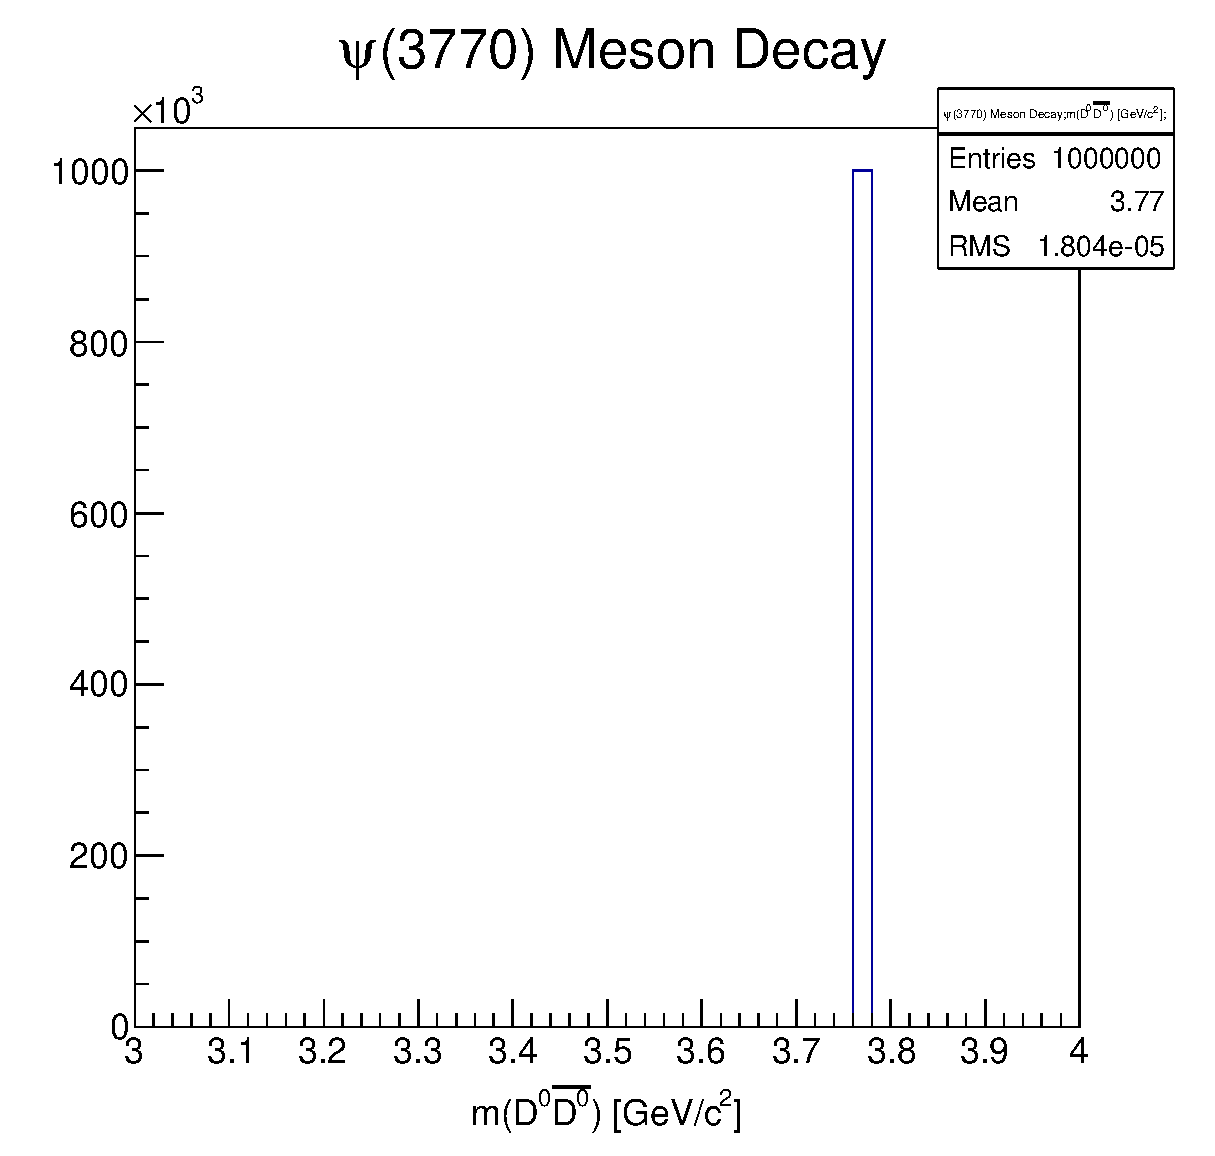
\includegraphics[scale=0.3]{graphs/TwoBodyDecay.eps}
\end{center}
\end{frame}

\subsection{Three body $B^+ \rightarrow D^0 \xbar{D^0}K^+$}

\begin{frame}{Three body $B^+ \rightarrow D^0 \xbar{D^0}K^+$}

Three bodies, so more complicated (and prettier):

\begin{center}
    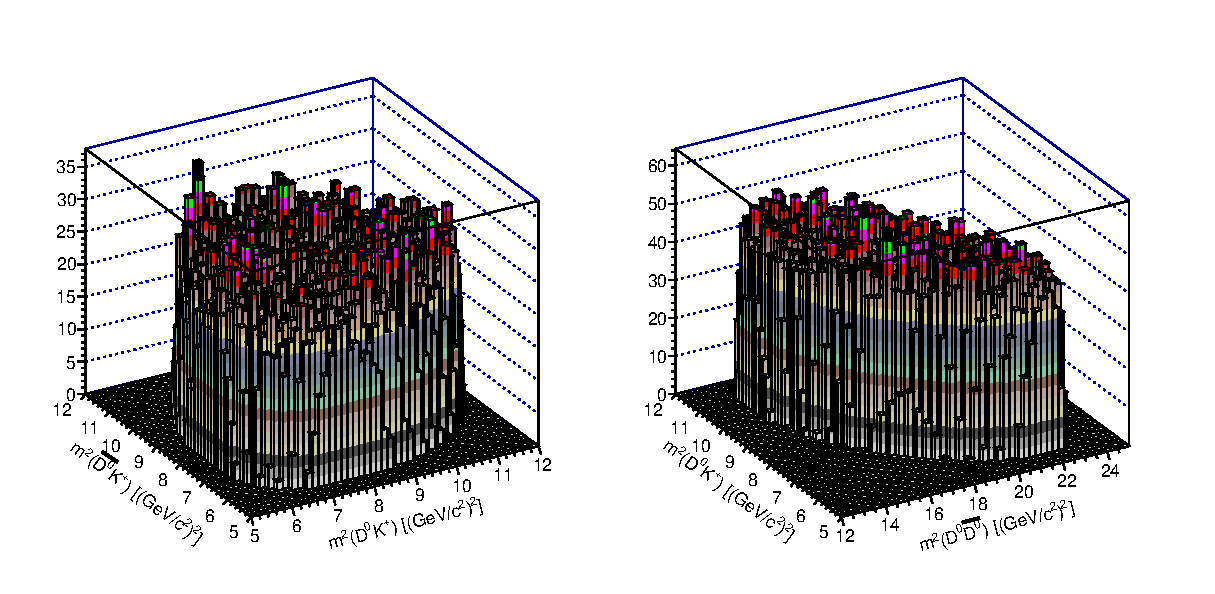
\includegraphics[width=\linewidth]{graphs/ThreeBodyDecay1.eps}
\end{center}
\end{frame}

\begin{frame}{Three body $B^+ \rightarrow D^0 \xbar{D^0}K^+$}
\begin{itemize}

    \Item A three body decay has a two-dimensional phase space, so this is best
        visualised as a density plot of the invariant mass distributions of
        combinations of two of the particles.
    
    \Item They are not unique and can be inferred from one another due to
        momentum conservation laws.
    
    \Item If there were no intermediate resonances in the decay, this should
        decay roughly uniformly throughout the phase space, meaning given if
        this MC were repeated an infinite number of times, the distribution
        would be approximately flat-topped.  Considering the finite number of
        iterations made, this isn't bad!
    
    \Item An example of an intermediate resonance in this decay that we are very
        interested in is $B \rightarrow \psi(3770) K$, which is not simulated
        here but which we will look at later.

\end{itemize}
\end{frame}

\subsection{Four body $D^0 \rightarrow K^+ K^- K^- \pi^+$}

\begin{frame}{Four body $D^0 \rightarrow K^+ K^- K^- \pi^+$}
\begin{itemize}

    \Item Also looked at phase space for uniform four body decays.
    
    \Item These produce five dimensional phase space, which is hard to
        visualise.  I've just projected these onto axes to turn them into 1D
        projections which \textbf{can} easily be plotted and understood.
    
    \Item (If you want to know more about visualising multi-dimensional phase
        spaces, talk to Dan Saunders.)

\end{itemize}
\end{frame}

\begin{frame}{Four body $D^0 \rightarrow K^+ K^- K^- \pi^+$}

\begin{center}
    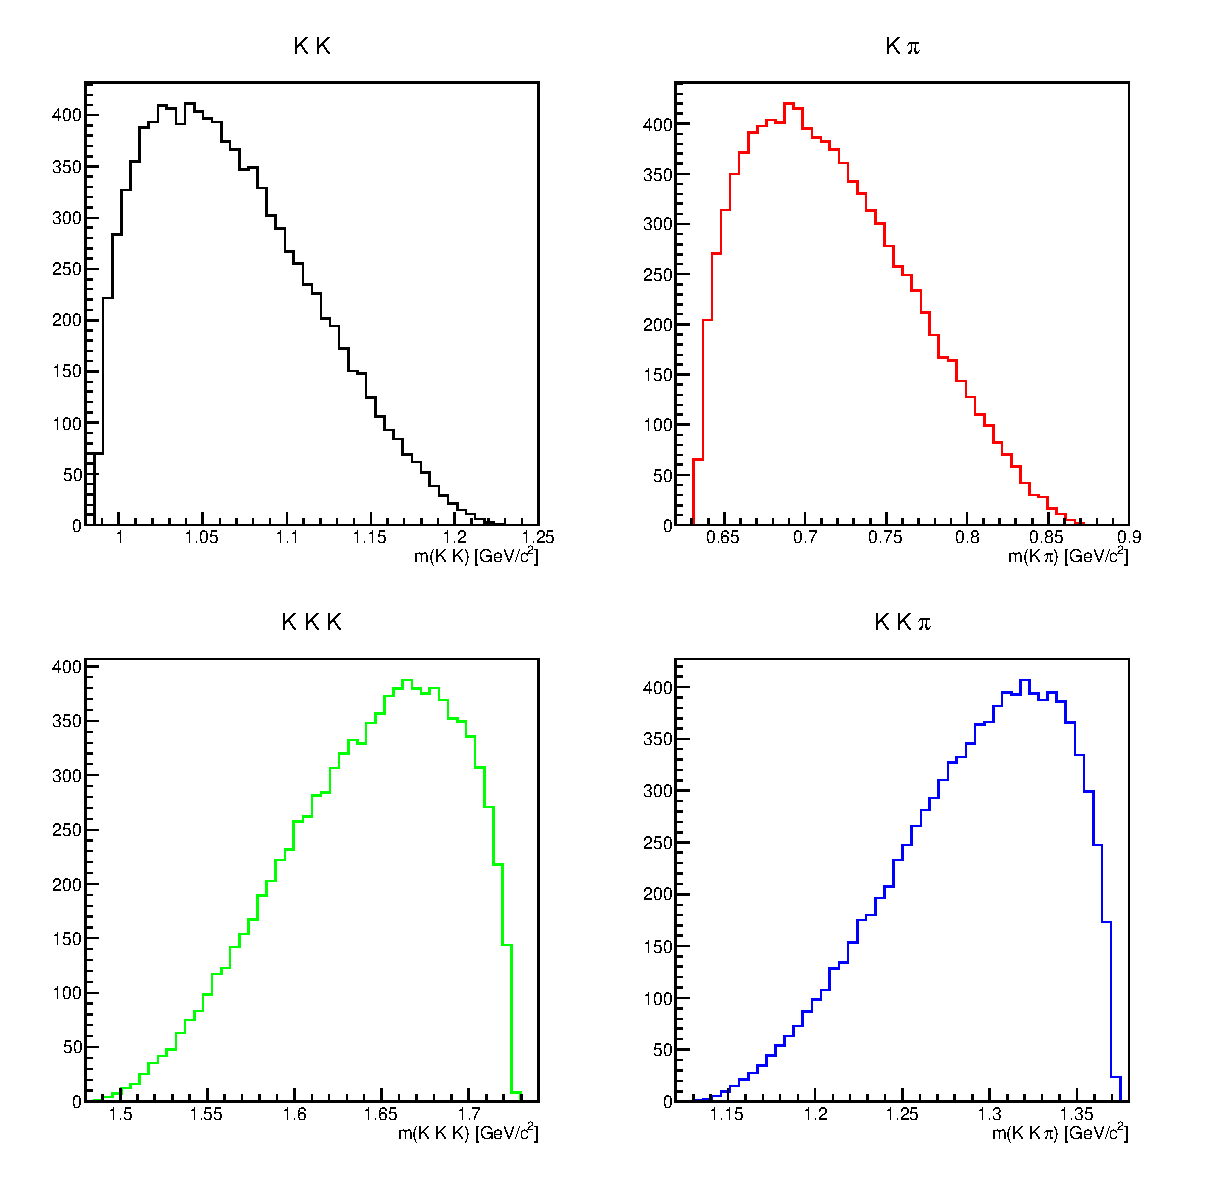
\includegraphics[scale=0.3]{graphs/FourBodyDecay.eps}
\end{center}
\end{frame}

\begin{frame}{Four body $D^0 \rightarrow K^+ K^- K^- \pi^+$}
\begin{itemize}

    \Item If I had simulated intermediate resonances in the decay we would see
        rich strong phase information arising from the interference between
        these decays.
    
    \Item If you're interested in this, the structure of such decays using
        ``Dalitz Plot Analysis'' has been done by Bristol's particle physics
        team for $D^0 \rightarrow K K \pi \pi$ deacys, and Jack Benton is now
        doing a Dalitz plot analysis of $D \rightarrow \pi \pi \pi \pi$ decays.
    
    \Item The $D^0 \rightarrow K^+ K^- K^- \pi^+$ decay strong phase information
        has never been observed! For interest, I tabulated the possible
        intermediate resonances:

\end{itemize}
\end{frame}

\begin{frame}
\tiny
{\centering
\begin{table}[H]
  \begin{tabu}{|[1.25pt] l |[1.25pt] p{1.5cm} |[1.25pt] p{2cm} |[1.25pt] l |[1.25pt] p{4cm} |[1.25pt]}
    \multicolumn{5}{c}{\Large{Light Unflavored Mesons} \large{($S=C=B=0$)}} \\
    \tabucline[1.25pt]{-}
    Particle Name & Mass [MeV] & Full width, $\Gamma$ [MeV] & $J^P$ & Decay
    Channel \\
    \tabucline[1.25pt]{-}
  
    $f_0(980)$ & 980 $\pm$ 10 & 40 $\rightarrow$ 100 & $0^+$ & 
      $f_0(980) \rightarrow K \xbar{K}$ 
    \\\hline
  
    $a_0(980)$ & 980 $\pm$ 20 & 50 $\rightarrow$ 100 & $0^+$ & 
      $a_0(980) \rightarrow K \xbar{K}$  
    \\\hline
  
    $\phi(1020)$ & 1019.45 $\pm$ 0.02 & 4.26 $\pm$ 0.04 & $1^-$ & 
      $\phi(1020) \rightarrow K^+K^-$  
    \\\hline
  
    $b_1(1235)$ & 1229.5 $\pm$ 3.2 & 142 $\pm$ 9 & $1^+$ &
      $b_1(1235) \rightarrow [\phi \rightarrow K^+ K^-] \pi$  \hfill and
      $b_1(1235) \rightarrow [K^*(892)^{\pm} \rightarrow K \pi]K^{\pm}$
    \\\hline
  
    $a_1(1260)$ & 1230 $\pm$ 40 & 250 $\rightarrow$ 600 & $1^+$ &
      $a_1(1260) \rightarrow [f_0(1370) \rightarrow K\xbar{K}]\pi$ \hfill and
      $a_1(1260) \rightarrow [f_2(1270) \rightarrow K\xbar{K}]\pi$ \hfill and
      $a_1(1260) \rightarrow K [\xbar{K}^*(892) \rightarrow K \pi] + c.c.$ 
    \\\hline
  
    $f_2(1270)$ & 1275.1 $\pm$ 1.2 & $185.1^{+2.9}_{-2.4}$ & $2+$ & 
      $f_2(1270) \rightarrow K\xbar{K}$
    \\\hline
  
    $f_1(1285)$ & 1281.8 $\pm$ 0.6 & 24.3 $\pm$ 1.1 & $1^+$ &
      $f_1(1285) \rightarrow K\xbar{K}\pi$
    \\\hline
  
    $\eta(1295)$ & 1294 $\pm$ 4 & 55 $\pm$ 5 & $0^-$ &
      $\eta(1295) \rightarrow a_0(980)\pi$
    \\\hline
  
    $a_2(1320)$ & 1318.3 $\pm$ 0.6 & 107 $\pm$ 5 & $2^+$ &
      $a_2(1320) \rightarrow K \xbar{K}$ 
    \\\hline
  
    $f_0(1370)$ & 1200 $\to$ 1500 & 200 $\to$ 500 & $0^+$ &
      $f_0(1370) \rightarrow K\xbar{K}$ 
    \\\hline
  
    $\eta(1405)$ & 1409.8 $\pm$ 2.5 & 51.1 $\pm$ 3.4 & $0^-$ &
      $\eta(1405) \rightarrow [a_0(980) \rightarrow K \xbar{K}] \pi$ \hfill and
      $\eta(1405) \rightarrow K \xbar{K} \pi$ \hfill and
      $\eta(1405) \rightarrow [K^*(892) \rightarrow K \pi] K$
    \\\hline
  
    $f_1(1420)$ & 1426.4 $\pm$ 0.9 & 54.9 $\pm$ 2.6 & $1^+$ & 
      $f_1(1420) \rightarrow K \xbar{K} \pi$ \hfill and
      $f_1(1420) \rightarrow K [\xbar{K}^*(892) \rightarrow K \pi] + c.c.$
    \\\hline
  
    $a_0(1450)$ & 1474 $\pm$ 19 & 265 $\pm$ 13 & $0^+$ & 
      $a_0(1450) \rightarrow K \xbar{K}$ 
    \\\hline
  
    $\rho(1450)$ & 1465 $\pm$ 13 & 265 $\pm$ 13 & $0^+$ & 
      $\rho(1450) \rightarrow K [\xbar{K}^*(892) \rightarrow K \pi] + c.c.$
      %(Possibly seen.)
    \\\hline
  
    $\eta(1475)$ & 1476 $\pm$ 4 & 85 $\pm$ 9 & $0^-$ &
      $\eta(1475) \rightarrow K \xbar{K} \pi$  \hfill and
      $\eta(1475) \rightarrow [a_0(980) \rightarrow K \xbar{K}] \pi$ \hfill and 
      $\eta(1475) \rightarrow K [\xbar{K}^*(892) \rightarrow K \pi] + c.c.$
    \\\hline
  
    $f_0(1500)$ & 1505 $\pm$ 6 & 109 $\pm$ 7 & $0^+$ &
      $f_0(1500) \rightarrow K \xbar{K}$
    \\\hline
  
    $f^{\prime}_2(1525)$ & 1525 $\pm$ 5 & $73^{+6}_{-5}$ & $2^+$ &
      $f^{\prime}_2(1525) \rightarrow K \xbar{K}$
    \\\hline

    \tabucline[1.25pt]{-}
  \end{tabu}
\end{table}
  
% vim: set filetype=tex:

}
\end{frame}

\begin{frame}
\tiny
{\centering
\begin{table}[H]
  \begin{tabu}{|[1.25pt] l |[1.25pt] p{1.5cm} |[1.25pt] p{2cm} |[1.25pt] l |[1.25pt] p{4cm} |[1.25pt]}
    \multicolumn{5}{c}{\Large{Light Unflavored Mesons} \large{($S=C=B=0$)}} \\
    \tabucline[1.25pt]{-}
    Particle Name & Mass [MeV] & Full width, $\Gamma$ [MeV] & $J^P$ & Decay
    Channel \\
    \tabucline[1.25pt]{-}

    $\eta_2(1645)$ & 1617 $\pm$ 5 & 181 $\pm$ 11 & $2^-$ &
      $\eta_2(1645) \rightarrow [a_2(1320) \rightarrow K \xbar{K}] \pi$ \hfill and
      $\eta_2(1645) \rightarrow K \xbar{K} \pi$ \hfill and
      $\eta_2(1645) \rightarrow [K^*(892) \rightarrow K \pi] \xbar{K}$ \hfill and
      $\eta_2(1645) \rightarrow [a_0(980) \rightarrow K \xbar{K}] \pi$
    \\\hline
  
    $\pi_2(1670)$ & 1672.2 $\pm$ 3.0 & 260 $\pm$ 9 & $2^-$ &
      $\pi_2(1670) \rightarrow [f_2(1270) \rightarrow K \xbar{K}] \pi$ \hfill and
      $\pi_2(1670) \rightarrow K [\xbar{K}^*(892) \rightarrow K \pi] + c.c.$
    \\\hline
  
    $\phi(1680)$ & 1680 $\pm$ 20 & 150 $\pm$ 50 & $1^-$ &
      $\phi(1680) \rightarrow K \xbar{K}$ \hfill and
      $\phi(1680) \rightarrow K [\xbar{K}^*(892) \rightarrow K \pi] + c.c.$
    \\\hline
  
    $\rho_3(1690)$ & 1688.8 $\pm$ 2.1 & 161 $\pm$ 10 & $3^-$ &
      $\rho_3(1690) \rightarrow K \xbar{K} \pi$ \hfill and
      $\rho_3(1690) \rightarrow K \xbar{K}$ \hfill and
      $\rho_3(1690) \rightarrow [a_2(1320) \rightarrow K \xbar{K}] \pi$
    \\\hline
  
    $\rho(1700)$ & 1720 $\pm$ 20 \newline ($\eta\rho^0$ \& $\pi^+\pi^-$) 
    %\footnote{$\eta\rho^0$ and $\pi^+\pi^-$ modes}
    %\addtocounter{footnote}{-1} \addtocounter{Hfootnote}{-1}
    %& 250 $\pm$ 100 \footnotemark{} & $1^-$ &
    & 250 $\pm$ 100 \newline ($\eta\rho^0$ \& $\pi^+\pi^-$) & $1^-$ &
      $\rho(1700) \rightarrow K \xbar{K}$ \hfill and
      $\rho(1700) \rightarrow K [\xbar{K}^*(892) \rightarrow K \pi] + c.c.$
    \\\hline
  
    $f_0(1710)$ & 1720 $\pm$ 6 & 135 $\pm$ 8 & $0^+$ &
      $f_0(1710) \rightarrow K \xbar{K}$
    \\\hline
  
    $\pi(1800)$ & 1812 $\pm$ 12 & 208 $\pm$ 12 & $0^-$ &
      $\pi(1800) \rightarrow [K^*(892) \rightarrow K \pi] K^-$
    \\\hline
  
    $\phi_3(1850)$ & 1854 $\pm$ 7 & $87^{+28}_{-23}$ & $3^-$ &
      $\phi_3(1850) \rightarrow K \xbar{K}$ \hfill and
      $\phi_3(1850) \rightarrow K [\xbar{K}^*(892) \rightarrow K \pi] + c.c.$
    \\\hline
  
    $f_2(1950)$ & 1944 $\pm$ 12 & 472 $\pm$ 18 & $2^+$ &
      $f_2(1950) \rightarrow K \xbar{K}$
    \\\hline
  
    $f_2(2010)$ & $2011^{+60}_{-80}$ & 202 $\pm$ 60 & $2^+$ &
      $f_2(2010) \rightarrow K \xbar{K}$
    \\\hline
  
    $a_4(2040)$ & $1996^{+10}_{-9}$ & $255^{+28}_{-24}$ & $4^+$ &
      $a_4(2040) \rightarrow K \xbar{K}$ \hfill and
      $a_4(2040) \rightarrow [f_2(1270) \rightarrow K \xbar{K}] \pi$
    \\\hline
  
    $f_4(2050)$ & 2018 $\pm$ 11 & 237 $\pm$ 18 & $4^+$ & 
      $f_4(2050) \rightarrow K \xbar{K}$ \hfill and
      $f_4(2050) \rightarrow [a_2(1320) \rightarrow K \xbar{K}] \pi$
    \\\hline
  
    $f_2(2300)$ & 2297 $\pm$ 28 & 149 $\pm$ 40 & $2^+$ &
      $f_2(2300) \rightarrow K \xbar{K}$
    \\
  
    \tabucline[1.25pt]{-}
  \end{tabu}
\end{table}
% vim: set filetype=tex:

}
\end{frame}

\begin{frame}
\tiny
{\centering
{\centering
\begin{table}[H]
  \begin{tabu}{|[1.25pt] l |[1.25pt] l |[1.25pt] l |[1.25pt] l |[1.25pt] p{6cm} |[1.25pt]}
    \multicolumn{5}{c}{\Large{Strange Mesons} \large{($S=\pm1, C=B=0$)}} \\
    \tabucline[1.25pt]{-}
    Particle Name & Mass [MeV] & Full width, $\Gamma$ [MeV] & $J^P$ & Decay
    Channel \\
    \tabucline[1.25pt]{-}
  
    $K^*(892)$ & 895.5 $\pm$ 0.8 & 46.2 $\pm$ 1.3 & $1^-$ &
      \multirow{3}{*}{$K^*(892) \rightarrow K \pi$}
    \\\cline{1-4}
  
    $K^*(892)^{\pm}$ & 891.66 $\pm$ 0.26 & 50.8 $\pm$ 0.9 & $1^-$ &
    \\\cline{1-4}
  
    $K^*(892)^0$ & 895.94 $\pm$ 0.22 & 48.7 $\pm$ 0.8 & $1^-$ &
    \\\hline
  
    $K_1(1270)$ & 1272 $\pm$ 7 & 90 $\pm$ 20 & $1^+$ &
      $K_1(1270) \rightarrow K [f_0(1370) \rightarrow K \xbar{K}]$
    \\\hline
  
    $K_1(1400)$ & 1403 $ \pm$ 7 & 174 $\pm$ 13 & $1^+$ &
      $K_1(1400) \rightarrow K [f_0(1370) \rightarrow K \xbar{K}]$
    \\\hline
  
    $K^*(1410)$ & 1414 $\pm$ 15 & 232 $\pm$ 21 & $1^-$ &
      $K^*(1410) \rightarrow K \pi$
    \\\hline
  
    $K^*_0(1430)$ & 1425 $\pm$ 50 & 270 $\pm$ 80 & $0^+$ &
      $K^*_0(1430) \rightarrow K \pi$
    \\\hline
  
    $K^*_2(1430)^{\pm}$ & 1425.6 $\pm$ 1.5 & 98.5 $\pm$ 2.7 & $2^+$ &
      \multirow{2}{*}{$K^*_2(1430) \rightarrow K \pi$}
    \\\cline{1-4}
  
    $K^*_2(1430)^0$ & 1432.4 $\pm$ 1.3 & 109 $\pm$ 5 & $2^+$ &
    \\\hline
  
    $K^*(1680)$ & 1717 $\pm$ 27 & 322 $\pm$ 110 & $1^-$ & 
      $K^*(1680) \rightarrow K \pi$
    \\\hline
  
    $K_2(1770)$ & 1773 $\pm$ 8 & 186 $\pm$ 14 & $2^-$ &
      $ K_2(1770) \rightarrow K [f_2(1270 \rightarrow K \xbar{K}] $ \hfill and
      $ K_2(1770) \rightarrow K [\phi \rightarrow K^+ K^-]$
    \\\hline
  
    $K^*_3(1780)$ & 1776 $\pm$ 7 & 159 $\pm$ 21 & $3^-$ &
      $ K^*_3(1780) \rightarrow K \pi $
    \\\hline
  
    $K_2(1820)$ & 1816 $\pm$ 13 & 276 $\pm$ 35 & $2^-$ &
      $ K_2(1820) \rightarrow K [f_2(1270) \rightarrow K \xbar{K}] $
    \\\hline
  
    $K^*_4(2045)$ & 1045 $\pm$ 9 & 198 $\pm$ 30 & $4^+$ &
      $ K^*_4(2045) \rightarrow K \pi $
    \\
  
    \tabucline[1.25pt]{-}
  \end{tabu}
  \captionof{table}{Table of possible resonances for the strange mesons.}
  \label{tab:StrangeMesons}
\end{table}
}

}
\end{frame}
